\section{Comparative analysis}
\label{analysis}

We carried out an extensive evaluation of the three state of the art design techniques for efficient model computation.
%: a) Model Compression via pruning redundant parameters and nodes, b) Quantization to lower the precision of model parameters and activations, and c) Efficient off-the-shelf architectures.
%
%We show that ... In addition, we show that ... 
We first describe the datasets and architectures used in this analysis in Section~\ref{datasets} before to present the considered metrics in Section~\ref{metrics}. Finally, we analyse efficiency Section~\ref{eval-efficiency} and privacy leakage Section~\ref{eval-leakage}.


\subsection{Datasets and Architectures}
\label{datasets}

For evaluating and comparing different efficiency algorithms, we use three simple datasets: FashionMNIST, Purchase100 and Location.
For Location and Purchase100 datasets, we train the model for 50 epochs while for FashionMNIST dataset we train the model for 75 epochs. 
%These provide us with the necessary direction to choose the optimal efficiency algorithm which satisfies all the efficiency and privacy requirement as describes in Section~\ref{motivate}.

\noindent\textbf{FashionMNIST.} This dataset consists of 60,000 training examples and a test set of 10,000 examples.
Each data record is a 28$\times$28 grayscale image which is mapped to one of 10 classes consisting of fashion products such as coat, sneaker, shirt, shoes.
For this dataset, we use a modified LeNet architecture with two convolution layers followed by maxpool and dense layers: [Conv 32 (3,3), Conv 64 (3,3), Maxpool (2,2), Dense 128, Dense 10] (Architecture 1). Additionally, we use a fully connected model [512,512,512] (Architecture 2).

\noindent\textbf{Purchase100.} This dataset is a privacy sensitive dataset capturing the purchase preferences of online customers taken from the authors of~\cite{shokri2017membership}.
The data records have 600 binary features and each record is classified into one of 100 classes identifying each user's purchase.
For this dataset, we use a fully connected architecture with the nodes in each layers as [1024,512,256,128,100].

\noindent\textbf{Location.} This dataset is a privacy sensitive dataset capturing user's location "check-ins" taken from the authors of~\cite{shokri2017membership} where each record has 446 binary features which is mapped to one of 30 classes each representing a location. For this dataset we use a fully connected architecture with hyperparameters as [512,256,128,30].




\subsection{Metrics}
\label{metrics}

\paragraph{Efficiency} We evaluate efficiency of the three baseline algorithms based on Memory efficiency, Computation efficiency and Energy efficiency. Memory efficiency is compared based on the reduction in the memory footprint of the model computed from the parameters stored in the memory. Computation efficiency is compared based on the reduction in the MAC operations which influences the execution time. Finally, the energy consumption is compared based on memory accesses from reading inputs and writing results to the memory. Since, significant literature has compared the efficiency empirically, we provide a qualitative comparison for the baseline algorithms.

\paragraph{Privacy}
We use the inference attack accuracy to estimate the success of membership inference attack.
An accuracy above random guess $50\%$ indicates a training data leakage through membership inference attack.
This indicates that the adversary is able to identify the membership details of a data record with an accuracy higher than random guess.
The success of inference attack accuracy is strongly correlated with the model's extent of overfitting empirically measured as the difference between the train and test accuracy (generalization error). Higher generalization error (overfitting) results in higher distinguishability between the test and train resulting in higher membership inference accuracy~\cite{shokri2017membership}.
Additionally, the accuracy of the model is computed using the model's performance on unseen test data.





%\subsection{Optimization for Efficiency}
\subsection{Evaluating Efficiency}
\label{eval-efficiency}

Here, in the view of the above efficiency requirements, we compare the three baseline algorithms.
We then select an efficient design scheme for NNs that satisfies all our requirements.


\noindent\textbf{Memory Efficiency.} Off the shelf models are designed to specifically reduce the memory footprint.
For instance, the memory footprint of Squeezenet and MobileNet is 5MB and 14Mb compared to 250Mb of Alexnet and >500Mb of VGG architectures.
Additionally, lowering the model precision from 64 or 32 bit floating point to binary precision results in a direct reduction of 64x or 32x in the overall memory footprint of the model.
However, in case of model compression the model parameters which are pruned are simply replaced by a value of "0".
Hence, storing even the "0" parameter takes up memory and does not necessarily decrease the overall memory footprint unless the hardware is optimized to skip the storage of all the zero values in the memory.
This requires additional logic to check for zero valued parameters in a dictionary.

\begin{figure*}[ht!]
\begin{center}% note that \centering uses less vspace...
\resizebox{2\columnwidth}{!}{%
\begin{tabular}{lllll}


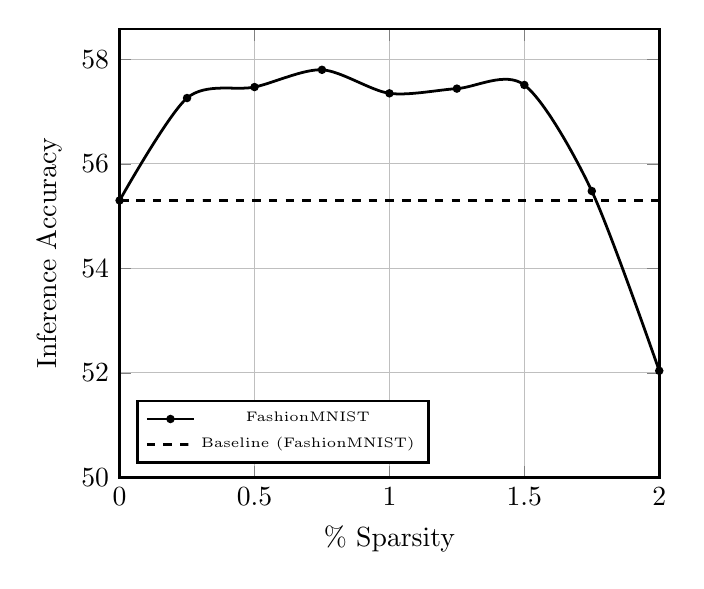
\begin{tikzpicture}
\begin{axis}[
legend style={font=\tiny},
legend pos =  south west,
line width=1.0pt,
mark size=1.0pt,
ymin=50,
xmin=0,
xmax=2,
legend entries={FashionMNIST, Baseline (FashionMNIST)},
ylabel={Inference Accuracy},
xlabel={\% Sparsity},
% extra x ticks={1,10,...,400},
% extra y ticks={0,0.5,...,10},
% extra y tick labels={},
% extra x tick labels={},
% extra x tick style={grid=major},
% extra y tick style={grid=major},
grid=major
]
\addplot[
    color=black,
    solid,
    mark=*,
    mark options={solid},
    smooth
    ]
    coordinates {
    (0,55.30)(0.25,57.26)(0.5,57.47)(0.75,57.80)(1,57.35)(1.25,57.44)(1.5,57.51)(1.75,55.48)(2,52.04)
      };
\addplot[
    color=black,
    dashed,
    smooth
    ]
    coordinates {
    (0,55.30)(0.25,55.30)(0.5,55.30)(0.75,55.30)(1,55.30)(1.25,55.30)(1.5,55.30)(1.75,55.30)(2,55.30)
      };
\end{axis}
\end{tikzpicture} &


%
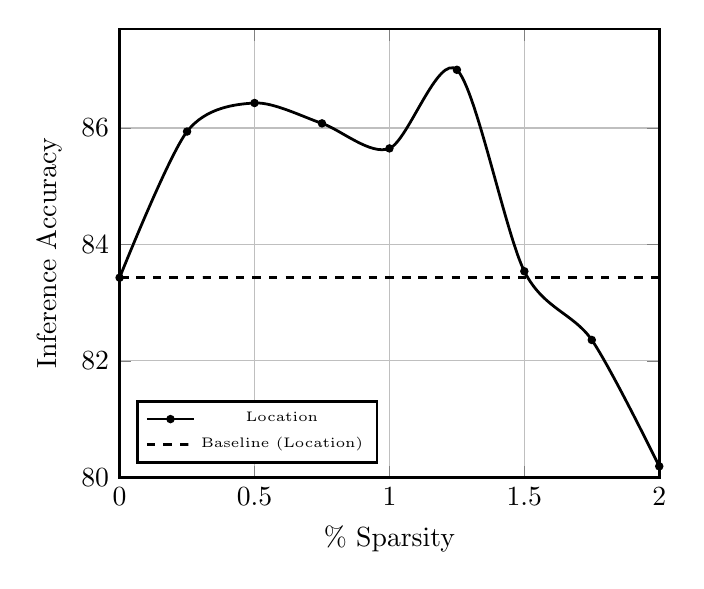
\begin{tikzpicture}
\begin{axis}[
legend style={font=\tiny},
legend pos =  south west,
line width=1.0pt,
mark size=1.0pt,
ymin=80,
xmin=0,
xmax=2,
legend entries={Location, Baseline (Location)},
ylabel={Inference Accuracy},
xlabel={\% Sparsity},
grid=major
]
\addplot[
    color=black,
    solid,
    mark=*,
    mark options={solid},
    smooth
    ]
    coordinates {
    (0,83.43)(0.25,85.94)(0.5,86.43)(0.75,86.08)(1,85.65)(1.25,87.00)(1.5,83.54)(1.75,82.36)(2,80.19)
      };
\addplot[
    color=black,
    dashed,
    smooth
    ]
    coordinates {
    (0,83.43)(0.25,83.43)(0.5,83.43)(0.75,83.43)(1,83.43)(1.25,83.43)(1.5,83.43)(1.75,83.43)(2,83.43)
      };

\end{axis}
\end{tikzpicture} &





%
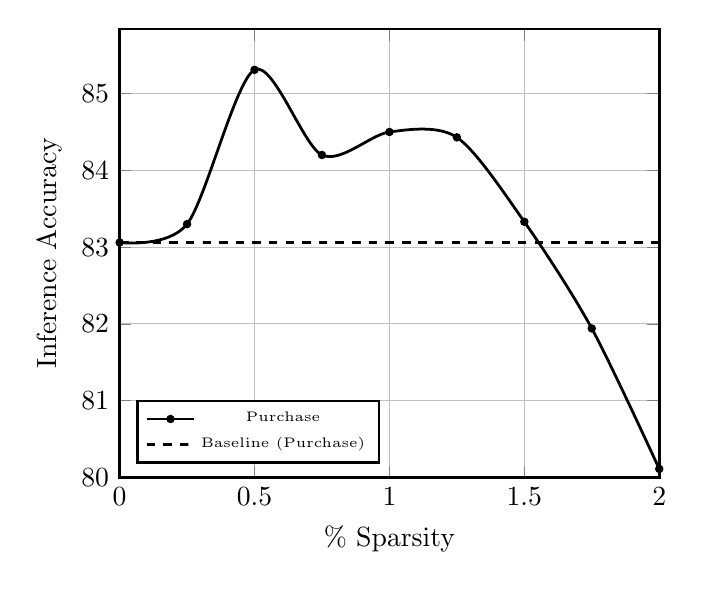
\begin{tikzpicture}
\begin{axis}[
legend style={font=\tiny},
legend pos =  south west,
line width=1.0pt,
mark size=1.0pt,
ymin=80,
xmin=0,
xmax=2,
legend entries={Purchase, Baseline (Purchase)},
ylabel={Inference Accuracy},
xlabel={\% Sparsity},
grid=major
]
\addplot[
    color=black,
    solid,
    mark=*,
    mark options={solid},
    smooth
    ]
    coordinates {
    (0,83.06)(0.25,83.30)(0.5,85.31)(0.75,84.20)(1,84.50)(1.25,84.43)(1.5,83.33)(1.75,81.94)(2,80.11)
      };
\addplot[
    color=black,
    dashed,
    smooth
    ]
    coordinates {
    (0,83.06)(0.25,83.06)(0.5,83.06)(0.75,83.06)(1,83.06)(1.25,83.06)(1.5,83.06)(1.75,83.06)(2,83.06)
      };

\end{axis}
\end{tikzpicture}


\end{tabular}
}
\caption{.}
\label{fig:loss}
\end{center}
\end{figure*}

\begin{figure*}[ht!]
\begin{center}% note that \centering uses less vspace...
\resizebox{2\columnwidth}{!}{%
\begin{tabular}{lllll}


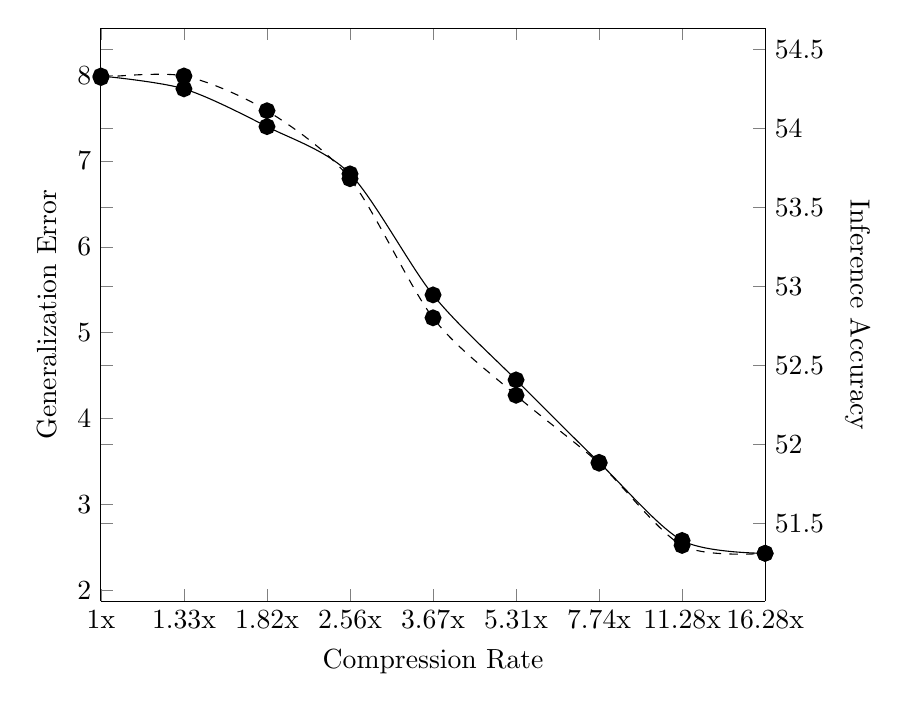
\begin{tikzpicture}
% let both axes use the same layers
\pgfplotsset{set layers}
%
\begin{axis}[
scale only axis,
line width=2.0pt,
mark size=2.0pt,
xmin=0,xmax=8,
ylabel={Generalization Error},
axis y line*=left,
xlabel={Compression Rate},
xtick={0,1,2,3,4,5,6,7,8},
xticklabels={1x, 1.33x, 1.82x, 2.56x, 3.67x, 5.31x, 7.74x, 11.28x, 16.28x}
]
\addplot[
    color=black,
    solid,
    mark=*,
    mark options={solid},
    smooth
    ]
    coordinates {
    (0,7.99)(1,7.84)(2,7.4)(3,6.85)(4,5.44)(5,4.45)(6,3.49)(7,2.58)(8,2.43)
      };
\end{axis}

\begin{axis}[
scale only axis,
line width=2.0pt,
mark size=2.0pt,
xmin=0,xmax=8,
ylabel near ticks, yticklabel pos=right,
ylabel={Inference Accuracy},
ylabel style = {rotate=180},
axis x line=none
]
\addplot[
    color=black,
    dashed,
    mark=*,
    mark options={solid},
    smooth
    ]
    coordinates {
    (0,54.32)(1,54.33)(2,54.11)(3,53.68)(4,52.80)(5,52.31)(6,51.88)(7,51.36)(8,51.31)
        };
\end{axis}
\end{tikzpicture} &

%
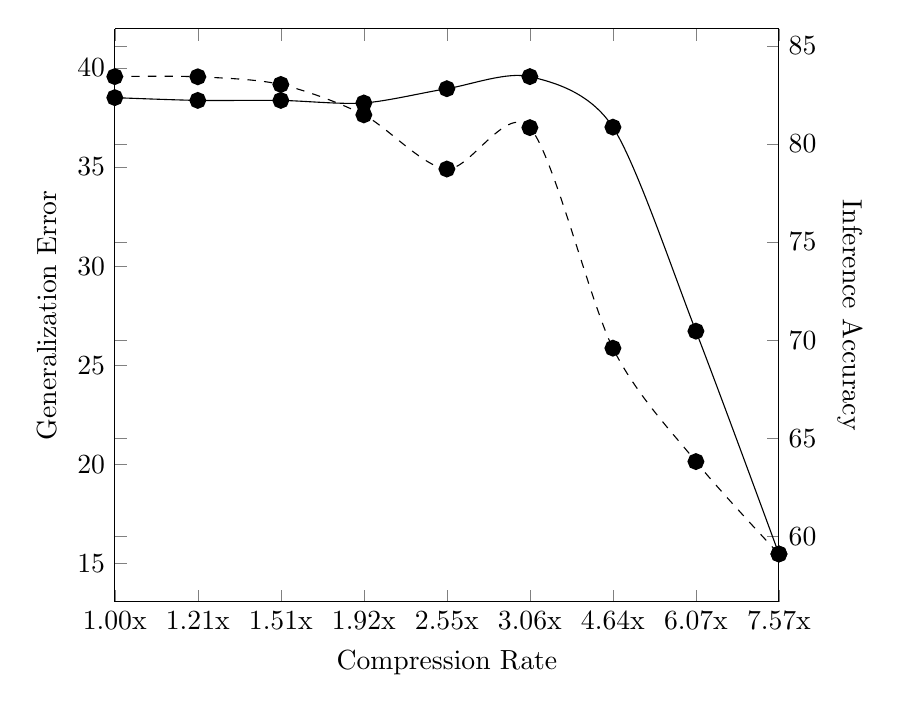
\begin{tikzpicture}
% let both axes use the same layers
\pgfplotsset{set layers}
%
\begin{axis}[
scale only axis,
line width=2.0pt,
mark size=2.0pt,
xmin=0,xmax=8,
ylabel={Generalization Error},
axis y line*=left,
xlabel={Compression Rate},
xtick={0,1,2,3,4,5,6,7,8},
xticklabels={1.00x, 1.21x, 1.51x, 1.92x, 2.55x, 3.06x, 4.64x, 6.07x, 7.57x}
]
\addplot[
    color=black,
    solid,
    mark=*,
    mark options={solid},
    smooth
    ]
    coordinates {
    (0,38.5)(1,38.36)(2,38.36)(3,38.23)(4,38.95)(5,39.56)(6,37.01)(7,26.72)(8,15.48)
      };
\end{axis}

\begin{axis}[
scale only axis,
line width=2.0pt,
mark size=2.0pt,
xmin=0,xmax=8,
ylabel near ticks, yticklabel pos=right,
ylabel={Inference Accuracy},
ylabel style = {rotate=180},
axis x line=none
]
\addplot[
    color=black,
    dashed,
    mark=*,
    mark options={solid},
    smooth
    ]
    coordinates {
    (0,83.43)(1,83.42)(2,83.03)(3,81.48)(4,78.72)(5,80.83)(6,69.59)(7,63.81)(8,59.10)
        };
\end{axis}
\end{tikzpicture} &





%
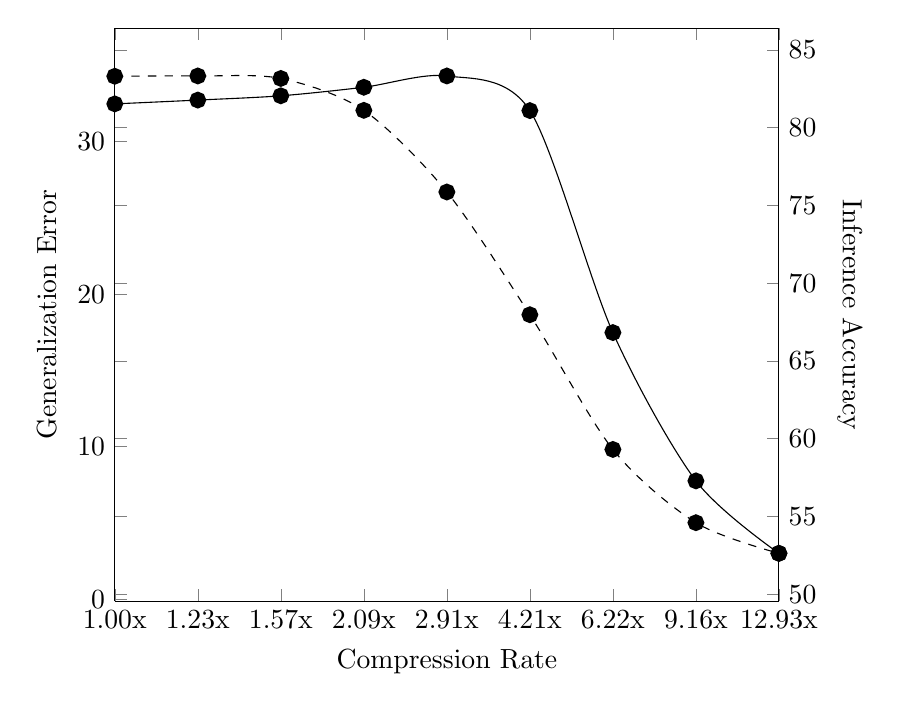
\begin{tikzpicture}
% let both axes use the same layers
\pgfplotsset{set layers}
%
\begin{axis}[
scale only axis,
line width=2.0pt,
mark size=2.0pt,
xmin=0,xmax=8,
ylabel={Generalization Error},
axis y line*=left,
xlabel={Compression Rate},
xtick={0,1,2,3,4,5,6,7,8},
xticklabels={1.00x, 1.23x, 1.57x, 2.09x, 2.91x, 4.21x, 6.22x, 9.16x, 12.93x}
]
\addplot[
    color=black,
    solid,
    mark=*,
    mark options={solid},
    smooth
    ]
    coordinates {
    (0,32.47)(1,32.72)(2,33)(3,33.56)(4,34.3)(5,32.03)(6,17.48)(7,7.76)(8,3.01)
      };
\end{axis}

\begin{axis}[
scale only axis,
line width=2.0pt,
mark size=2.0pt,
xmin=0,xmax=8,
ylabel near ticks, yticklabel pos=right,
ylabel={Inference Accuracy},
ylabel style = {rotate=180},
axis x line=none
]
\addplot[
    color=black,
    dashed,
    mark=*,
    mark options={solid},
    smooth
    ]
    coordinates {
    (0,83.30)(1,83.32)(2,83.16)(3,81.11)(4,75.86)(5,67.97)(6,59.31)(7,54.60)(8,52.63)
        };
\end{axis}
\end{tikzpicture}


\end{tabular}
}
\caption{FashionMNIST(left) Purchase100(Center) Location(Right). Dashed is Inference accuracy, solid is generalisaton error}
\label{fig:loss}
\end{center}
\end{figure*}



\noindent\textbf{Computation Efficiency.} Design of efficient off-the-shelf architectures replaces the complex matrix-vector multiplications by multiple matrix-vector multiplications with smaller dimensions.
This reduces the overall number of parameters but it has been shown empirically\footnote{https://github.com/albanie/convnet-burden} that this does not necessarily reduce the number of multiply accumulate operations or FLOPS~\cite{article}.
In case of parameter pruning, achieving efficiency requires additional hardware optimization. Particularly, instead of actually computing the the multiplications with "0"pruned values, the hardware optimization enable the user to skip the computation and replace the output by a "0" directly.
For quantized models with binarized parameters and activations the MAC operations can be replaced by binary operations such as XNOR and the maxpool operations can be replaced by OR operation, while the activations can be replaced by checking the parity bit (denotes the sign) operation and hence reducing the FLOPS drastically~\cite{235489}.
This results in high computational efficiency and hence, faster inference.


\noindent\textbf{Energy Efficiency.} Energy efficiency has been shown to not vary much in case of reduction with number of parameters and data type, number of memory accesses play vital role~\cite{6757323}.
Specifically, for the case of off-the-shelf architectures the while the computation efficiency has been shown to improve, the energy efficiency has been shown to be close to large scale state of the art models like AlexNet~\cite{DBLP:journals/corr/IandolaMAHDK16,8114708}.
Alternatively, for the case of model compression, energy efficiency can be achieved by additionally providing hardware optimization and shows small improvement in the energy consumption~\cite{journals/corr/YangCS16a,DBLP:journals/corr/HanMD15}.
For quantization, however, the energy efficiency has been shown to be high where the memory access can be drastically reduced by increasing the throughput of data fetched from the memory.
Specifically, lowering the precision from 32 bit floating point to binary results in lowering the memory accesses and 32x improvement in energy consumption~\cite{NIPS2016_6573,rastegari2016xnornet}.
While some improvement is seen natively for quantized models (from replacing MACs with XNOR), higher benefits can be achieved via additional hardware optimization~\cite{Umuroglu2017FINNAF}.
The benchmarking of energy consumption for different optimization and architectures is well explored in the literature and out of scope of this work. We refer the authors to~\cite{8114708} for more details.

In summary, compared to different optimization techniques for NNs, the quantized architectures show significant benefit for different efficiency requirements over the other alternatives.




\subsection{Evaluating Privacy Leakage}
\label{eval-leakage}

In this section, we evaluate the information leakage through membership inference attacks for the three baseline algorithms considered.
This is the main contribution of our work where we evaluate the privacy leakage for different optimization and design algorithms for NNs.

\subsubsection{Model Compression}

We evaluate the privacy leakage on compressing a model by pruning the connections in the model.
Here, pruning is achieved by replacing some of the parameters with "0" value.
As described in the original paper~\cite{Han:2015:LBW:2969239.2969366,DBLP:journals/corr/HanPNMTECTD16}, pruning is followed by retraining the model to restore the model's original accuracy with the pruned connections.

We evaluate and validate the impact on membership privacy on compressing the model trained on three datasets: FashionMNIST, Location and Purchase100.
On pruning the model, the model's test accuracy decreases but also lowers the membership inference accuracy (Figure~\ref{fig:prune}).
This is expected as the parameters are responsible for memorizing the training data information~\cite{DBLP:journals/corr/abs-1812-00910,236216,10.1145/3133956.3134077} and pruning the parameters lowers the adversary's attack success.

\begin{figure*}[ht!]
\begin{center}% note that \centering uses less vspace...
\resizebox{2\columnwidth}{!}{%
\begin{tabular}{lllll}


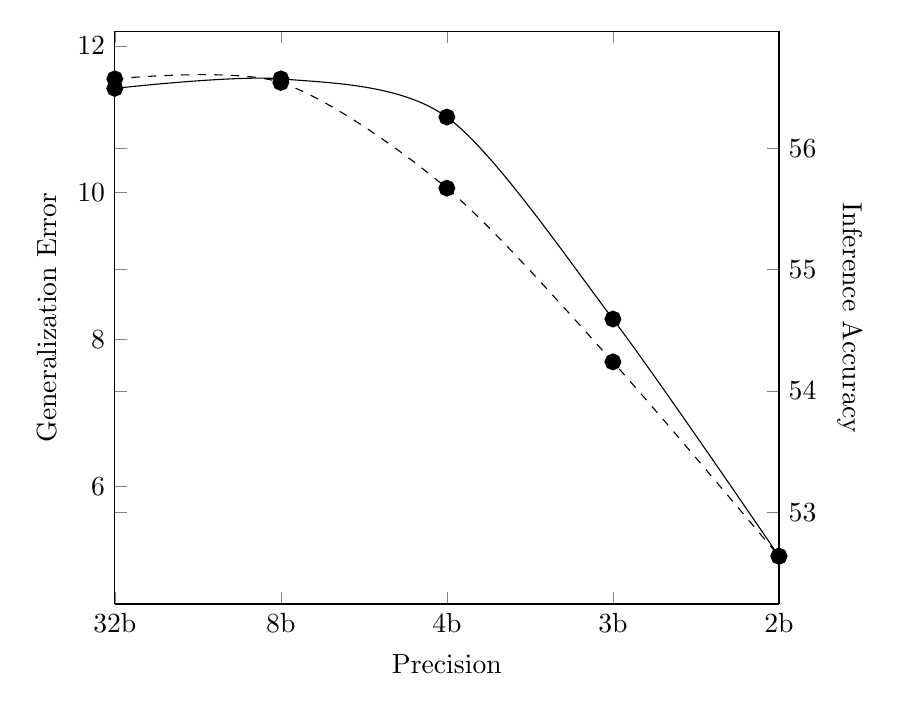
\begin{tikzpicture}
% let both axes use the same layers
\pgfplotsset{set layers}
%
\begin{axis}[
scale only axis,
line width=2.0pt,
mark size=2.0pt,
xmin=0,xmax=4,
ylabel={Generalization Error},
axis y line*=left,
xlabel={Precision},
xtick={0,1,2,3,4},
xticklabels={32b, 8b, 4b, 3b, 2b}
]
\addplot[
    color=black,
    solid,
    mark=*,
    mark options={solid},
    smooth
    ]
    coordinates {
    (0,11.42)(1,11.55)(2,11.03)(3,8.28)(4,5.05)
      };
\end{axis}

\begin{axis}[
scale only axis,
line width=2.0pt,
mark size=2.0pt,
xmin=0,xmax=4,
ylabel near ticks, yticklabel pos=right,
ylabel={Inference Accuracy},
ylabel style = {rotate=180},
axis x line=none
]
\addplot[
    color=black,
    dashed,
    mark=*,
    mark options={solid},
    smooth
    ]
    coordinates {
    (0,56.57)(1,56.54)(2,55.67)(3,54.24)(4,52.64)
        };
\end{axis}
\end{tikzpicture} &

%
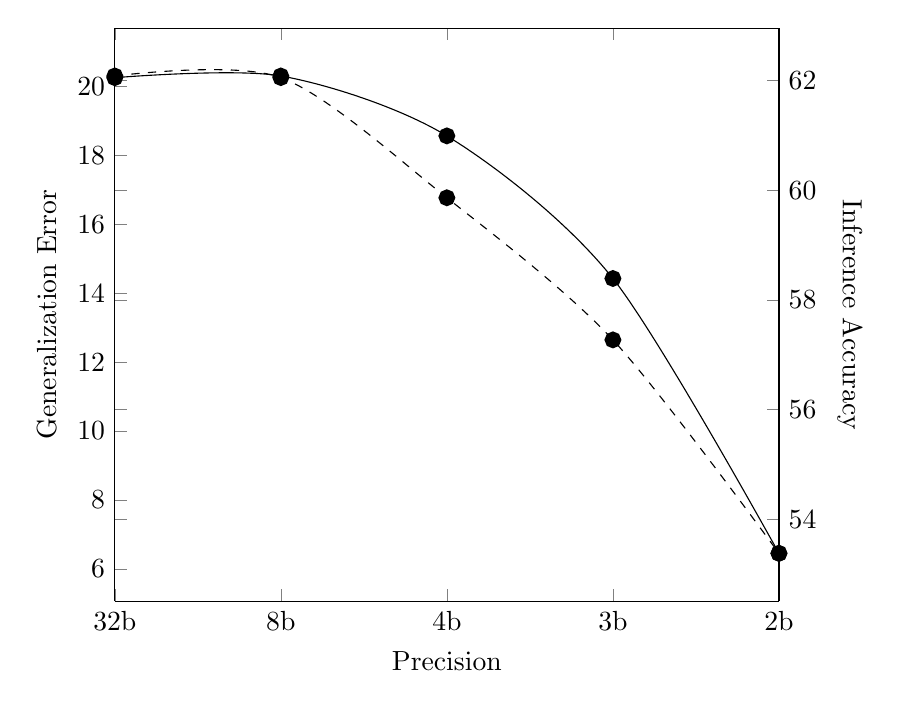
\begin{tikzpicture}
% let both axes use the same layers
\pgfplotsset{set layers}
%
\begin{axis}[
scale only axis,
line width=2.0pt,
mark size=2.0pt,
xmin=0,xmax=4,
ylabel={Generalization Error},
axis y line*=left,
xlabel={Precision},
xtick={0,1,2,3,4},
xticklabels={32b, 8b, 4b, 3b, 2b}
]
\addplot[
    color=black,
    solid,
    mark=*,
    mark options={solid},
    smooth
    ]
    coordinates {
    (0,20.26)(1,20.31)(2,18.57)(3,14.43)(4,6.45)
      };
\end{axis}

\begin{axis}[
scale only axis,
line width=2.0pt,
mark size=2.0pt,
xmin=0,xmax=4,
ylabel near ticks, yticklabel pos=right,
ylabel={Inference Accuracy},
ylabel style = {rotate=180},
axis x line=none
]
\addplot[
    color=black,
    dashed,
    mark=*,
    mark options={solid},
    smooth
    ]
    coordinates {
    (0,62.08)(1,62.05)(2,59.86)(3,57.27)(4,53.38)
        };
\end{axis}
\end{tikzpicture} &





%
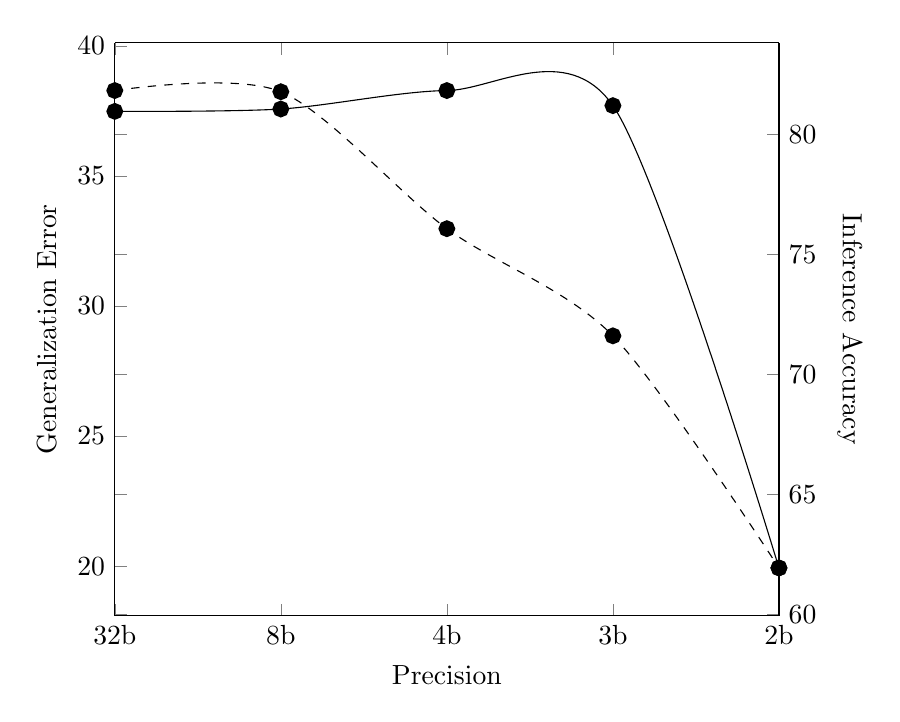
\begin{tikzpicture}
% let both axes use the same layers
\pgfplotsset{set layers}
%
\begin{axis}[
scale only axis,
line width=2.0pt,
mark size=2.0pt,
xmin=0,xmax=4,
ylabel={Generalization Error},
axis y line*=left,
xlabel={Precision},
xtick={0,1,2,3,4},
xticklabels={32b, 8b, 4b, 3b, 2b}
]
\addplot[
    color=black,
    solid,
    mark=*,
    mark options={solid},
    smooth
    ]
    coordinates {
    (0,37.48)(1,37.57)(2,38.28)(3,37.70)(4,19.93)
      };
\end{axis}

\begin{axis}[
scale only axis,
line width=2.0pt,
mark size=2.0pt,
xmin=0,xmax=4,
ylabel near ticks, yticklabel pos=right,
ylabel={Inference Accuracy},
ylabel style = {rotate=180},
axis x line=none
]
\addplot[
    color=black,
    dashed,
    mark=*,
    mark options={solid},
    smooth
    ]
    coordinates {
    (0,81.82)(1,81.77)(2,76.07)(3,71.61)(4,61.95)
        };
\end{axis}
\end{tikzpicture}


\end{tabular}
}
\caption{\underline{Pruning followed by Weight Sharing (Quantization).} While the retraining after pruning is necessary to restore the predictive accuracy, clustering the weights to reduce the precision lowers the inference accuracy (dashed line) risk while reducing the generalization error (solid line) for FashionMNIST(left), Purchase100(Center) and Location(Right) dataset.}
\label{fig:loss}
\end{center}
\end{figure*}


However, interestingly, on retraining the pruned model, we observe that the membership inference accuracy is much higher than the original unpruned baseline model (Figure~\ref{fig:retrain}).
This indicates that model compression in turn increases the overall privacy leakage.
This can be attributed to the lower number of parameters forced to learn the same amount of information stored previously in the unpruned model with larger number of parameters.
In other words, the same amount of information is now captured by less number of parameters resulting in higher memorization of information per parameter.
As the model is compressed (pruned), the number of parameters decreases which results in increase in information per parameter. However, on aggressive pruning, the train accuracy also decreases resulting in a decrease in the information per parameter, which is empirically indicated by a decrease in membership inference accuracy at the end in (Figure~\ref{fig:retrain}).
%To analyze the information stored per parameter, we first compute the model capacity as the mutual information of a trained network between the true label $Y$ and the predicted label $Y_{\theta}$ for a random input $X$ as derived in~\cite{45932,cap}.
%Here, model's information $I(Y;Y_{\theta}|X) = $
%\begin{equation}
%\footnotesize
%N_{train}\left(1 - (r_{train}log_2(\frac{1}{r_{train}}) + (1-r_{train})log_2(\frac{1}{1-r_{train}}))\right)
%\end{equation}
%where $r_{train}$ is the classification train accuracy for all the $N_{train}$ samples in the training data.
%For $r_{train} = 1$, the model completely memorizes all random samples as the information stored equals the number of samples $N_{train}$, while for $r_{train}=0.5$, the training accuracy 0.
%We divide the above equation by the model's total number of parameters $N_{param}$ to get the per parameter information stored as
%\begin{equation}
%I_p(Y;Y_{\theta}|X) = \frac{I(Y;Y_{\theta}|X)}{N_{param}}
%\end{equation}



\textbf{Mitigating the Privacy Risks in Pruned Models.} We describe on potential approach to mitigate the privacy risk of the compressed models without requiring to modify the model's training.
The post-hoc approach utilizes the weight sharing for the compressed model. This is however, accompanied by a decrease in the model's prediction accuracy indicating a privacy-utility trade-off.
As seen in Figure~\ref{fig:wtsharing}, reducing the precision from 32 bits to 2 bits results in a decrease in inference accuracy from 56.57\% to 52.64\% for FashionMNIST, 62.08\% to 53.38\% for Purchase100 and 81.82\% to 61.95\% for Location dataset.
This decrease in inference attack accuracy is closely followed by a decrease in generalization error which is indicative of decrease in prediction accuracy of the model.
We evaluate the effectiveness of pruning followed by quantization which has been shown to have significant impact on reducing the model complexity through compression more significantly than either pruning or quantization alone.
For the experiments, we use the compressed model indicating highest privacy leakage to evaluate the effectiveness of weight sharing on the worst case condition.
This pipeline approach of pruning followed by retraining followed by weight sharing, not only maintains the algorithm's objective for efficiency but is used as a post-hoc approach to reduces the overall inference risk~\cite{DBLP:journals/corr/HanMD15,DBLP:journals/corr/HanPNMTECTD16}.






\subsubsection{Off-the-Shelf Efficient Architectures}


\begin{table}[!htb]
\begin{center}
\renewcommand\arraystretch{1.5}
\fontsize{6.7pt}{6.7pt}\selectfont
\begin{tabular}{|c|c|c|c|c|}
\hline
\textbf{Architecture} & \textbf{Memory} & \textbf{Train}  & \textbf{Test}  & \textbf{Inference}   \\
 & \textbf{Footprint} & \textbf{Accuracy} & \textbf{Accuracy} & \textbf{Accuracy}  \\
\hline
SqueezeNet & 5 MB & 88.21\% & 81.92\% & \cellcolor{green!25}53.07\% \\
MobileNetV2 & 14 MB & 97.50\% & 87.24\% & \cellcolor{green!25}55.57\% \\
\hline
AlexNet & 240 MB & 97.86\% & 80.34\% & \cellcolor{red!25}60.40\% \\
VGG11 & 507 MB & 99.13\% & 86.43\% & \cellcolor{red!25}58.04\% \\
VGG16 & 528 MB & 99.58\% & 88.95\% & \cellcolor{red!25}58.70\%  \\
VGG19 & 549 MB & 99.09\% & 88.18\% & \cellcolor{red!25}57.85\% \\
\hline
\end{tabular}
\end{center}
\caption{Model complexity influences the membership inference leakage.}
\label{stdarch}
\end{table}

In this section, we evaluate two popular state of the art architectures, SqueezeNet and MobileNet, trained on CIFAR10 dataset used for low powered systems.
As seen in Table~\ref{stdarch}, the SqueezeNet and MobileNet models shows lower inference accuracy of 53.07\% and 55.57\% compared to larger models which have higher privacy leakage.

\begin{figure}[hb!]
\resizebox{0.8\columnwidth}{!}{%
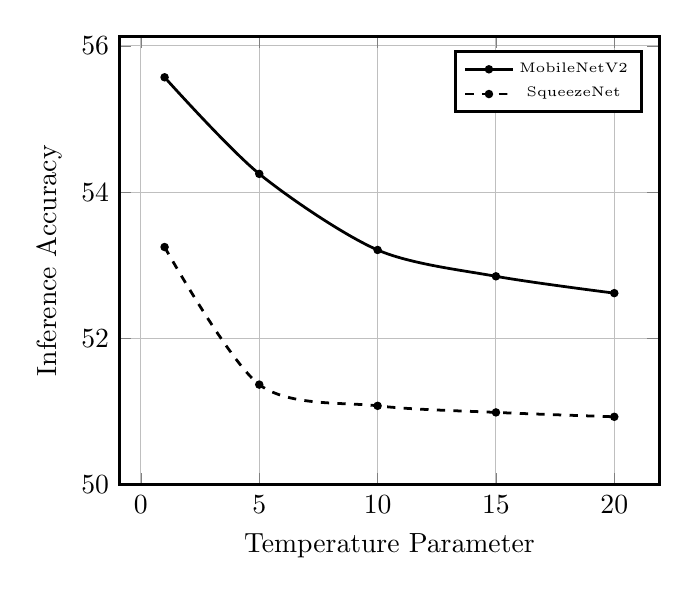
\begin{tikzpicture}
\begin{axis}[
legend style={font=\tiny},
legend pos =  north east,
line width=1.0pt,
mark size=1.0pt,
ymin=50,
legend entries={MobileNetV2, SqueezeNet},
ylabel={Inference Accuracy},
xlabel={Temperature Parameter},
% extra x ticks={1,10,...,400},
% extra y ticks={0,0.5,...,10},
% extra y tick labels={},
% extra x tick labels={},
% extra x tick style={grid=major},
% extra y tick style={grid=major},
grid=major
]
\addplot[
    color=black,
    solid,
    mark=*,
    mark options={solid},
    smooth
    ]
    coordinates {
    (1,55.57)(5,54.25)(10,53.21)(15,52.85)(20,52.62)
      };
\addplot[
      color=black,
      dashed,
      mark=*,
      mark options={solid},
      smooth
    ]
    coordinates {
    (1,53.25)(5,51.37)(10,51.08)(15,50.99)(20,50.93)
      };
\end{axis}
\end{tikzpicture}
}
\caption{The privacy leakage of models designed for efficiency (SqueezeNet and MobileNet) can be reduced by increasing the softmax temperature. }
\end{figure}


Further, the inference accuracy of SqueezeNet and MobileNet can be further reduced close to random guess by increasing the temperature parameter of the softmax function applied to the output.
Increasing the temperature parameter reduces the granularity of the model's output and is given by
$F_i(x) = e^{\frac{z_i(x)}{T}}$ / $ \sum_{j}e^{\frac{z_j(x)}{T}}$
%$F_i(x) = \frac{e^{\frac{z_i(x)}{T}}}{\sum_{j}e^{\frac{z_j(x)}{T}}}$ 
where $z(x)$ computes output of the model before the softmax layer.
For the case of SqueezeNet, we are able to reduce the inference accuracy to 50.93\% from 53.07\% while for MobileNet we can reduce the inference accuracy to 52.62\% from 55.57\% as seen in Figure~\ref{softmax}.
This reduction in inference accuracy is without any cost of the prediction test accuracy of the model.




\subsubsection{Quantization}

In this section, we evaluate the technique of reducing the precision of both model's parameters and intermediate activations.
Further, we consider the extreme case of binarizing the parameters and activations allowing to evaluate on the most optimized case.
We evaluate on FashionMNIST dataset for two architectures with convolutional and fully connected layers.

\begin{table}[!htb]
\begin{center}
\renewcommand\arraystretch{1.5}
\fontsize{6.7pt}{6.7pt}\selectfont
\begin{tabular}{|c|c|c|c|c|}
\hline
\multicolumn{5}{|c|}{\textbf{FashionMNIST}}\\
\hline
\textbf{Architecture} & \textbf{Memory} & \textbf{Train}  & \textbf{Test}  & \textbf{Inference}  \\
 & \textbf{Accuracy} &  \textbf{Footprint} & \textbf{Accuracy} & \textbf{Accuracy}  \\
\hline
\multicolumn{5}{|c|}{Architecture 1}\\
Full & 38.39 MB & 100\% & 92.35\% & \cellcolor{red!25}57.46\%\\
BinaryNet & 1.62 MB & 88.68\% & 86.9\% & \cellcolor{green!25}55.45\%\\
XNOR-Net & 1.62 MB & 87.19\% & 85.68\% & \cellcolor{green!25}51.05\%\\ %1,626,824 parameters
\hline
\multicolumn{5}{|c|}{Architecture 2}\\
Full & 29.83 MB & 99.34\% & 89.88\% & \cellcolor{red!25}54.86\% \\
BinaryNet & 0.93 MB & 97.61\% & 89.60\% & \cellcolor{green!25}54.30\%\\
XNOR-Net & 0.93 MB & 92.67\% & 86.68\% & \cellcolor{green!25}51.74\%\\ %937,000parameters
\hline
\end{tabular}
\end{center}
\caption{Reducing the model precision lowers the inference attack accuracy but at the cost of test accuracy.}
\label{fmnist_quantize}
\end{table}

In both the architectures, we see that computation on  binarized parameters and activations reduces the inference risk by a small value.
However, on replacing the MAC operations with XNOR operations, we observe that the inference risk decreases close to random guess, however, at the cost of prediction test accuracy.

In summary, we observe that quantization, specifically binarization of parameters and activation along with XNOR computation, provides strong resistance against inference attacks compared to model compression and off-the-shelf architectures.

\subsection{Summary of Comparison}

We summarize the properties satisfied by each of the technique in terms of privacy, computation, memory and energy efficiency in Table~\ref{tbl:comparison}.
Here, we mark the attributes which are satisfied with $\cmark$, requires additional hardware optimization as $\smark$ and does not satisfy the property with a $\xmark$.

\begin{table}[!htb]
\begin{center}
\renewcommand\arraystretch{1.5}
\fontsize{6.7pt}{6.7pt}\selectfont
\begin{tabular}{|l||l|l|l|}
\hline
Requirements & Compression & Quantization & Off-the-shelf  \\
\hline
Computation Efficiency & $\smark$  & $\cmark$   & $\xmark$ \\
\hline
Memory Efficiency &  $\smark$ & $\cmark$   & $\cmark$ \\
\hline
Energy Efficiency &  $\smark$   & $\cmark$   & $\xmark$ \\
\hline
Privacy &  $\xmark$   & $\cmark$   & $\smark$ \\
\hline
\end{tabular}
\end{center}
\caption{Only quantization satisfies all the requirements.}
%\caption{Comparison of different optimizations for NNs. $\smark$: additional hardware optimization; $\xmark$: requirement not satisfied; $\cmark$: requirement satisfied.}
\label{tbl:comparison}
\end{table}

In order to design NNs for embedded devices, quantization (binarization with XNOR computation) is an attractive design choice which not only satisfies the computation, memory and energy efficiency but also provides high resistance against inference attacks.
On the other hand, model compression leaks more training records membership details making it vulnerable to membership inference attacks. Additionally, it requires hardware support and optimization to achieve better efficiency. Off-the-shelf architectures, while provide decent privacy, does not provide satisfy all aspects of efficiency.
Hence, we choose quantization as a design for NNs to provide a good three dimensional trade-off between privacy-efficiency-accuracy.




